% LaTeX Template for short student reports.
% Citations should be in bibtex format and go in references.bib
\documentclass[a4paper, 11pt]{article}
\usepackage[top=3cm, bottom=3cm, left = 2.5cm, right = 2.5cm]{geometry}
\usepackage[english]{babel} 
\geometry{a4paper} 
\usepackage[utf8]{inputenc}
\usepackage{textcomp}
\usepackage{graphicx} 
\usepackage{amsmath,amssymb} 
\usepackage{mathtools} 
\usepackage{bm}  
\usepackage[hidelinks]{hyperref} 

\usepackage{setspace}
\onehalfspacing

\usepackage{pgfplots}
\pgfplotsset{width=10cm,compat=1.9}

\setlength{\parindent}{0cm}
%\hypersetup{linkcolor=black,citecolor=black,filecolor=black,urlcolor=black} % black links, for printed output
\usepackage{memhfixc} 
\usepackage{pdfsync}  
\usepackage{fancyhdr}
\pagestyle{fancy}

\usepackage[compact]{titlesec}  
\titlespacing*{\section}{0pt}{10ex plus 1ex minus .2ex}{4.3ex plus .2ex}

\usepackage[backend=biber, maxbibnames=99]{biblatex}

\addbibresource{references.bib}

\title{Runtime analysis of the Java implementation of the CYK-algorithm}
\author{Pina Kolling \\ piko0011@student.umu.se}
%\date{}


\newcommand{\dq}{"}






%---------------------------------------------------------------------%

%---------------------------------------------------------------------%






\begin{document}


\begin{titlepage}
	\centering
	{\scshape\LARGE Ume\r{a} University \par}
	Efficient Algorithms \par
	\vspace{1cm}
	{\scshape\Large Assignment Step 2 \par }
	\vspace{1.5cm}
	{\huge\bfseries  Runtime analysis of the Java implementation of the CYK-algorithm \par}
	\vspace{2cm}
	{\Large\itshape Pina Kolling\par}
	\vfill

% Bottom of the page
	{\large \today\par}
\end{titlepage}








%---------------------------------------------------------------------%







\setcounter{page}{1}


\newpage
\fancyhead[LO]{\empty}
{
  \hypersetup{linkcolor=black}
  \tableofcontents
}




\newpage





%---------------------------------------------------------------------%








\section{Introduction}

Parsing in Computer Science is the process of analysing a string of characters to examine if the string is built according to the rules of a formal grammar. \cite{CYK1}

A formal grammar describes how to form strings with correct syntax from a language's alphabet.
To examine if such a string follows the rules of a grammar the CYK-algorithm can be used. Therefore the grammar needs to be in a specific format, called CNF (explained in section \ref{CNF}).
\\ 
\\
The task for this assignment was to code three different parsing methods to execute the CYK-algorithm in \textit{Java}.
For this three different classes were implemented: \texttt{main.java, grammar.java} and \texttt{parser.java}. The \texttt{main}-class calls the methods and the \texttt{grammar}-class parses the input grammer ans string into a format that then can be processed in the \texttt{parser}-class.
The function and implementation will be former described in section \ref{systemdesign}.


\pagebreak






%---------------------------------------------------------------------%








\section{Background}

\begin{itemize}
\item grammar \\
A formal grammar describes how to form strings with correct syntax from a language's alphabet. A grammar does not describe the meaning of the strings or any semantics — only their syntax is defined.
\item CNF \label{CNF}
\item CYK
\item DP
\end{itemize}

\pagebreak





%---------------------------------------------------------------------%








\section{System Design}
\label{systemdesign}

My system worked as follows \ldots

\pagebreak






%---------------------------------------------------------------------%







\section{Evaluation}

We did some experiments \ldots

\pagebreak





%---------------------------------------------------------------------%








\section{Conclusions and Future Work}

From our experiments we can conclude that \ldots

\newpage





%---------------------------------------------------------------------%








\appendix

\section{How to use the code?}

The code can be run in the terminal and input is expected as Strings in quotation marks. The grammar needs to be in CNF. The first rule begins with the startsymbol of the grammar. \\ \\
First: Rules without arrows (one rule as one String) \\
Last: The last argument is the input word
\\ 

Input example (\textit{Well-Balanced-Parantheses}):\\
  \texttt{java Main \dq SSS\dq \ \dq SLA\dq \ \dq SLR\dq \ \dq ASR\dq \ \dq L(\dq \ \dq R)\dq\  \dq (())\dq}
\\ 
for the grammar \texttt{S $\rightarrow$ SS | LA | LR, A $\rightarrow$ SR, L $\rightarrow$ (, R $\rightarrow$ )} and the input word \texttt{(())}.
\\ \\
Output example: \\
The first part of the output shows the arrays, which get generated in the \texttt{Grammar.java} class.  \\ \\
\begin{minipage}{0.6\textwidth}
\vspace*{-2em}
The first array contains all rules. \\ \\ \\

The second array contains only the terminal rules. \\ \\

The third array contains only the nonterminal rules. \\

Then it is shown which nonterminal symbols are represented by which integers. Later the nonterminal symbols can be referred to with those integers. \\ 

After this the mentioned arrays are shown again but the nonterminal symbols got replaced with the according integers.

\end{minipage}\begin{minipage}{0.2\textwidth}
\ 
\end{minipage}\begin{minipage}{0.3\textwidth}
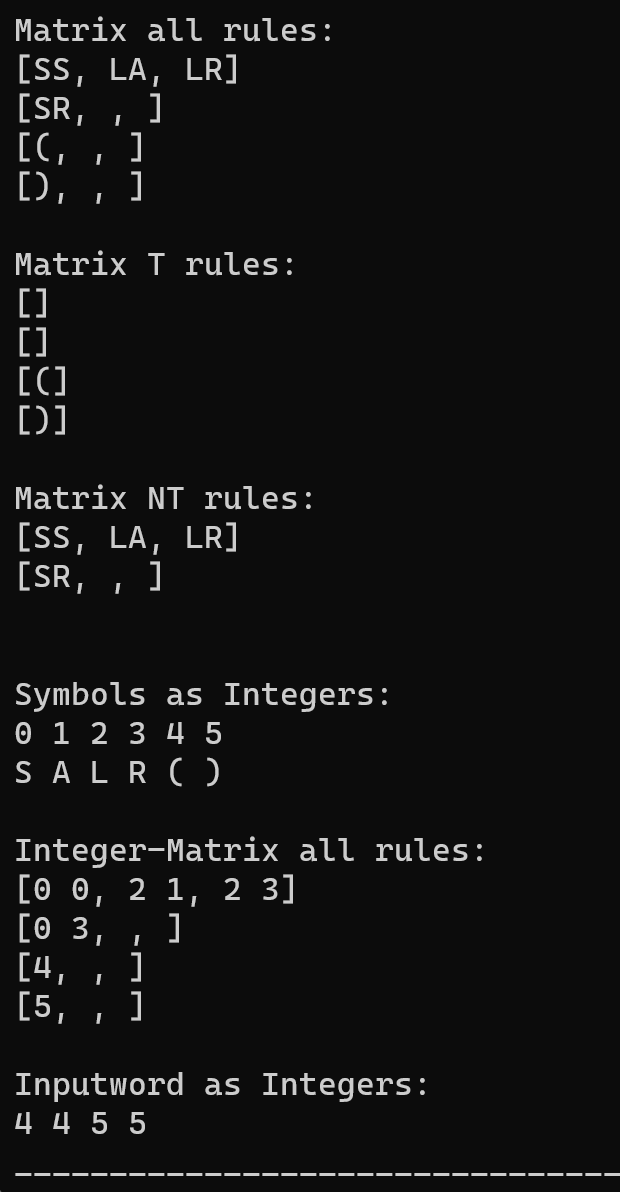
\includegraphics[scale=0.7]{images/terminal_1.png}
\end{minipage}

\begin{minipage}{0.4\textwidth}
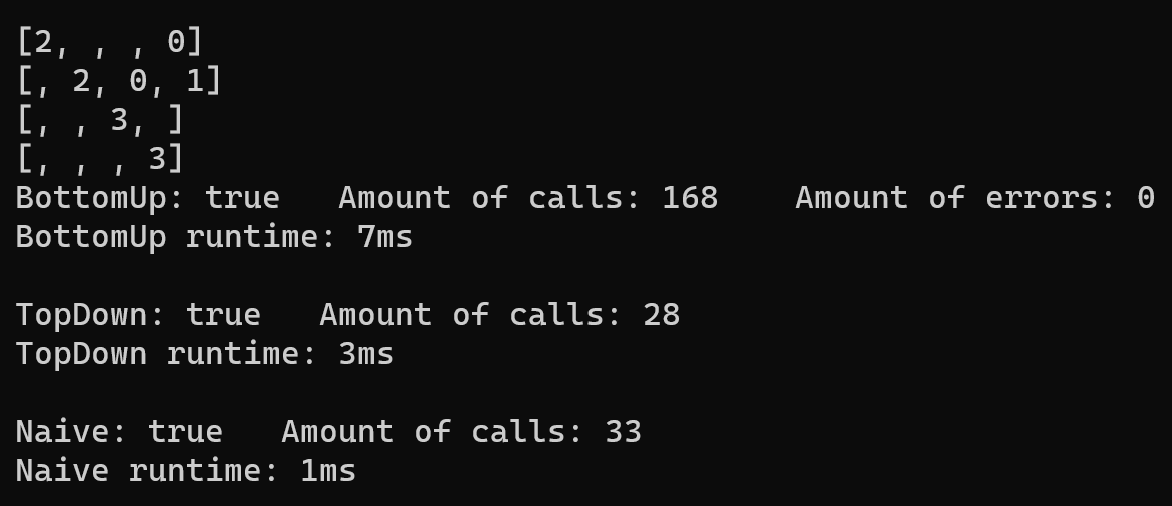
\includegraphics[scale=0.6]{images/terminal_2.png}
\end{minipage}\begin{minipage}{0.6\textwidth}
Then the results, counter and runtime in $ms$ is shown for each parsing method. \\
For the \texttt{BottomUp} method is the CYK algorithm table printed.
\end{minipage}









%---------------------------------------------------------------------%







\fancyhead[LO]{\empty}




\newpage
\phantomsection
\addcontentsline{toc}{section}{\bibname}
%\begin{spacing}{1.3}
\printbibliography
%\end{spacing}



\end{document}